\section{General Project Context}

In a rapidly evolving retail environment, the demand for seamless, secure, and efficient payment solutions has become increasingly critical—particularly in regions where digital transformation is accelerating but still faces structural challenges.

The \textbf{Credix} platform was conceived as a response to recurring issues identified in traditional Point of Sale (POS) systems, such as limited integration, manual transaction processing, and a lack of flexible credit management for businesses. Designed as a cross-platform mobile application with a robust backend architecture, Credix aims to modernize how transactions are initiated, processed, and monitored in real time across Tunisia's retail and food service sectors.

Beyond offering a simple digital payment method, the solution introduces features such as tokenized wallet-based payments, biometric authentication, credit allocation for corporate clients, and real-time barcode validation via direct integration with POS terminals. These enhancements are intended not only to streamline the customer experience but also to enable better control, visibility, and security for all stakeholders—vendors, employees, and enterprise clients alike.

The development of Credix relied on modern, scalable technologies—Flutter for the front-end mobile interface and Spring Boot for the back-end API layer—ensuring maintainability, performance, and ease of integration with existing ASM POS systems. It also takes into account regional requirements, including multilingual support (English, French, Arabic) and offline functionality in areas with unstable internet connectivity.

In essence, Credix serves as both a technical and strategic response to the current limitations of payment infrastructures in Tunisia, while paving the way for future enhancements such as loyalty programs, bill splitting, and intelligent credit recommendations.

\subsection{Problem Statement}

Despite increasing adoption of digital tools in the retail and restaurant sectors, many businesses in Tunisia still rely on fragmented payment systems that are ill-suited for modern transaction needs. Several recurring issues have been identified:

\begin{itemize}
    \item \textbf{Lack of integration between systems:} Businesses often juggle multiple tools for payment processing, credit allocation, and reporting, leading to inefficiencies and errors.

    \item \textbf{Manual processes and limited automation:} Many vendors still rely on partially manual operations\hspace{0pt}\textemdash\ especially for validating payments or managing employee credit balances—which increases the risk of delays and fraud.
    
    \item \textbf{Inflexible credit management:} Current POS platforms do not support corporate-specific credit rules, such as monthly limits, dynamic allocations, or centralized credit distribution.
    
    \item \textbf{Security concerns:} Traditional systems often lack modern authentication and fraud prevention mechanisms, making them vulnerable to misuse, particularly in high-volume retail contexts.
    
    \item \textbf{Poor user experience:} End users (employees) and vendors report friction in daily use—ranging from slow validation times to confusing interfaces and a lack of transparency in transaction histories.
\end{itemize}

These limitations hinder operational efficiency, reduce trust between businesses and their clients, and limit the ability to scale digitally. Addressing this context requires the development of a unified, secure, and flexible platform that:

\begin{itemize}
    \item Centralizes all core payment and credit management features;
    \item Automates key processes, including validation, fraud detection, and settlement;
    \item Offers a seamless and localized user experience across devices;
    \item Ensures compliance with both corporate policies and data protection standards.
\end{itemize}

The Credix solution was therefore designed to overcome these challenges through a tightly integrated mobile and backend system, tailored specifically to the needs of ASM’s partners and clients in the Tunisian market.


\subsection{Study and critique of existing systems}

In this section, we proceed with a critical analysis of digital payment and retail transaction applications available on the Tunisian and international markets. This comparative study aims to highlight the strengths of these solutions while emphasizing their limitations, in order to identify innovation opportunities for the development of Credix across diverse retail categories including restaurants, markets, boutiques, pharmacies, and other commercial establishments.

\clearpage
\subsubsection{National Solutions}

\begin{figure}[!htb]
    \centering
    \begin{subfigure}[b]{0.32\textwidth}
        \centering
        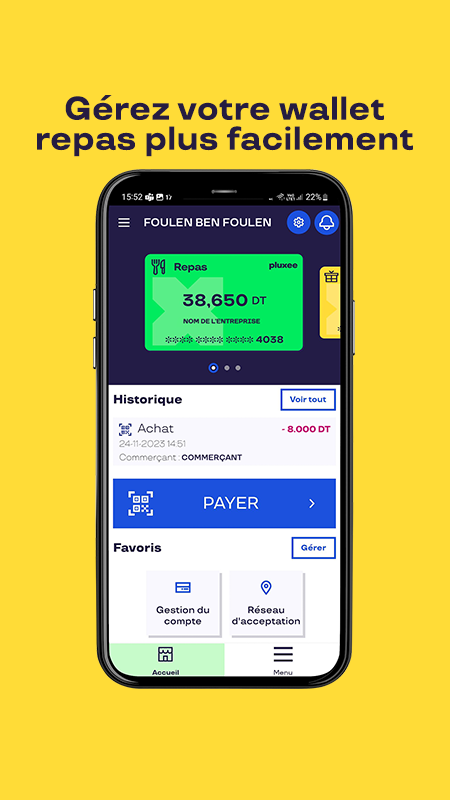
\includegraphics[width=\textwidth]{images/pluxee_screenshot_1.png}
        \caption{Pluxee Screenshot 1}
        \label{fig:pluxee_1}
    \end{subfigure}
    \hfill
    \begin{subfigure}[b]{0.32\textwidth}
        \centering
        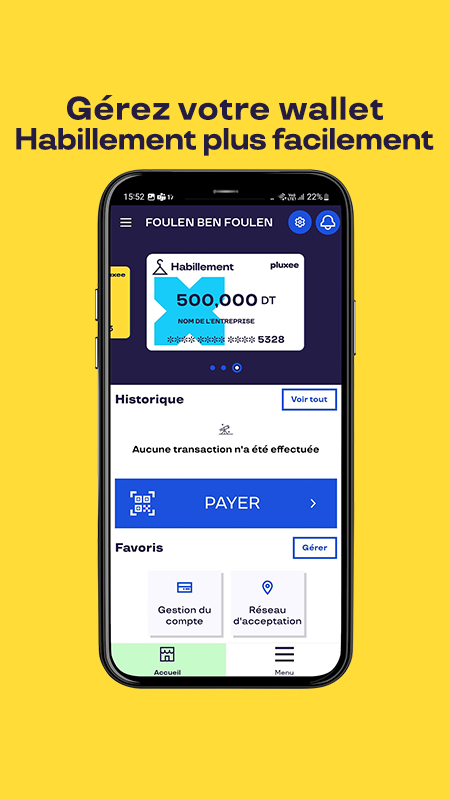
\includegraphics[width=\textwidth]{images/pluxee_screenshot_2.png}
        \caption{Pluxee Screenshot 2}
        \label{fig:pluxee_2}
    \end{subfigure}
    \hfill
    \begin{subfigure}[b]{0.32\textwidth}
        \centering
        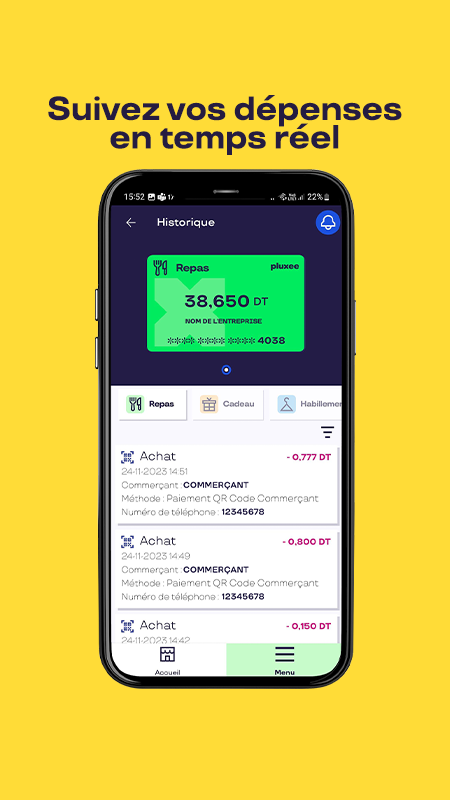
\includegraphics[width=\textwidth]{images/pluxee_screenshot_3.png}
        \caption{Pluxee Screenshot 3}
        \label{fig:pluxee_3}
    \end{subfigure}
    \caption{Pluxee Tunisia Interface}
    \label{fig:pluxee_interface}
\end{figure}

\textbf{Pluxee Tunisia:} (Figure~\ref{fig:pluxee_interface}) is a Tunisian application dedicated to digital meal vouchers and employee benefit management, offering a digital card for balance viewing, QR code payment functionality, and basic transaction history. It benefits from an established corporate client base and regulatory compliance with Tunisian financial authorities. However, it suffers from frequent application crashes and instability, which disrupts the payment process across retail establishments. It provides a limited and often inaccurate list of available vendors, restricting usage primarily to restaurants and excluding other retail categories like markets, boutiques, and pharmacies. The user interface is characterized by poor design and non-intuitive navigation, leading to a frustrating user experience. Furthermore, it lacks advanced corporate control features for employers, exhibits slow transaction processing times, and has minimal integration with diverse POS systems used across different retail sectors.

\clearpage

\begin{figure}[!htb]
    \centering
    \begin{subfigure}[b]{0.32\textwidth}
        \centering
        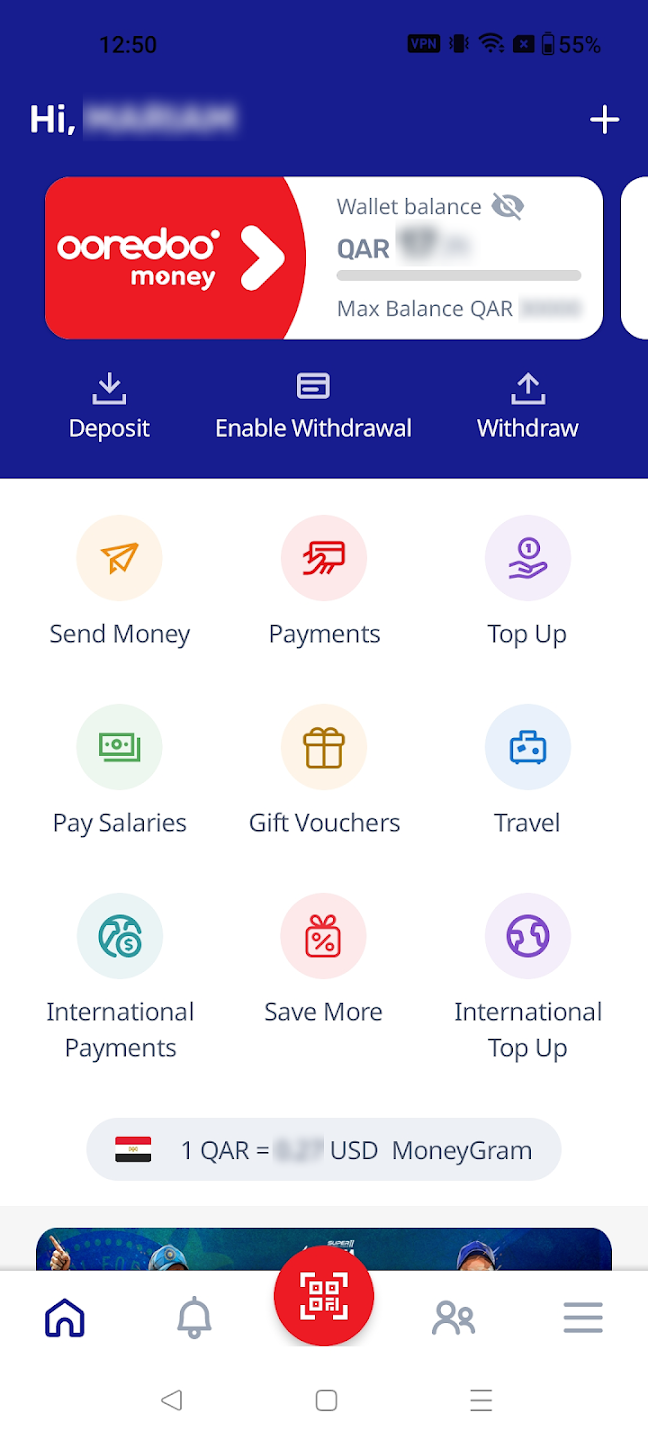
\includegraphics[width=\textwidth]{images/ooredoo_money_screenshot_1.png}
        \caption{Ooredoo Money Screenshot 1}
        \label{fig:ooredoo_1}
    \end{subfigure}
    \hfill
    \begin{subfigure}[b]{0.32\textwidth}
        \centering
        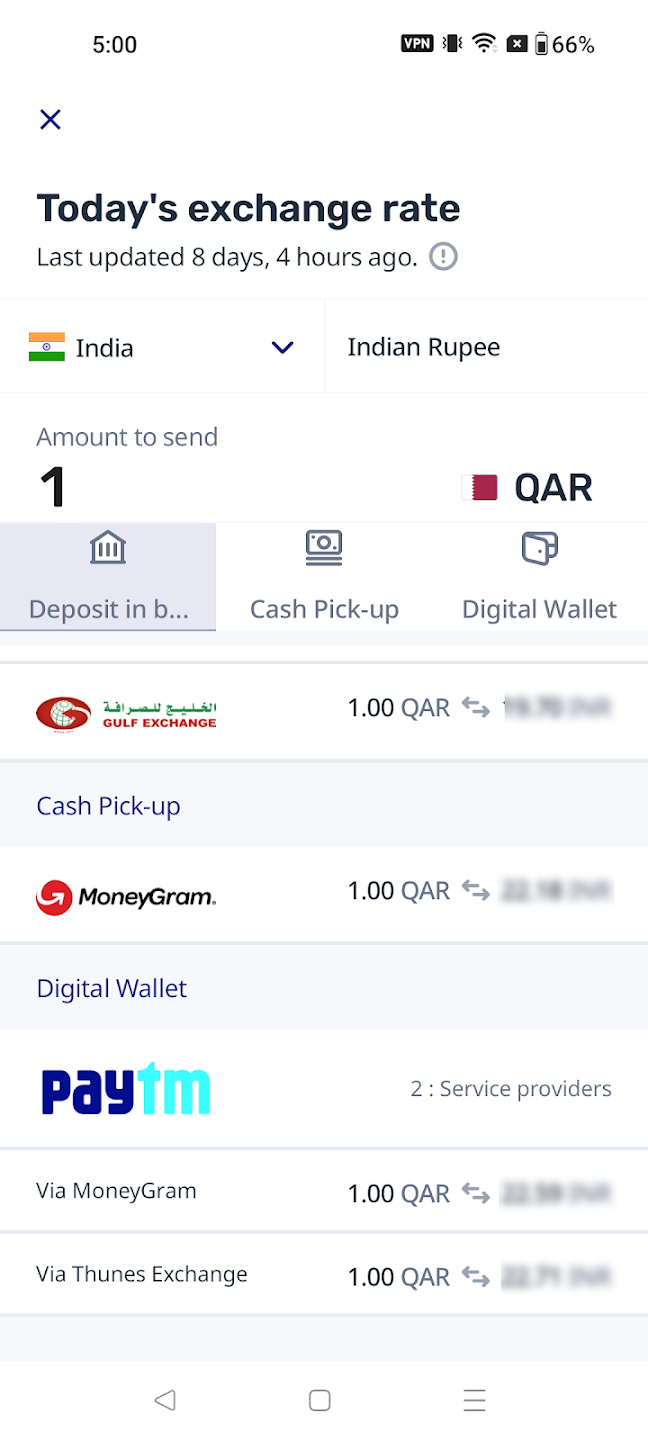
\includegraphics[width=\textwidth]{images/ooredoo_money_screenshot_2.png}
        \caption{Ooredoo Money Screenshot 2}
        \label{fig:ooredoo_2}
    \end{subfigure}
    \hfill
    \begin{subfigure}[b]{0.32\textwidth}
        \centering
        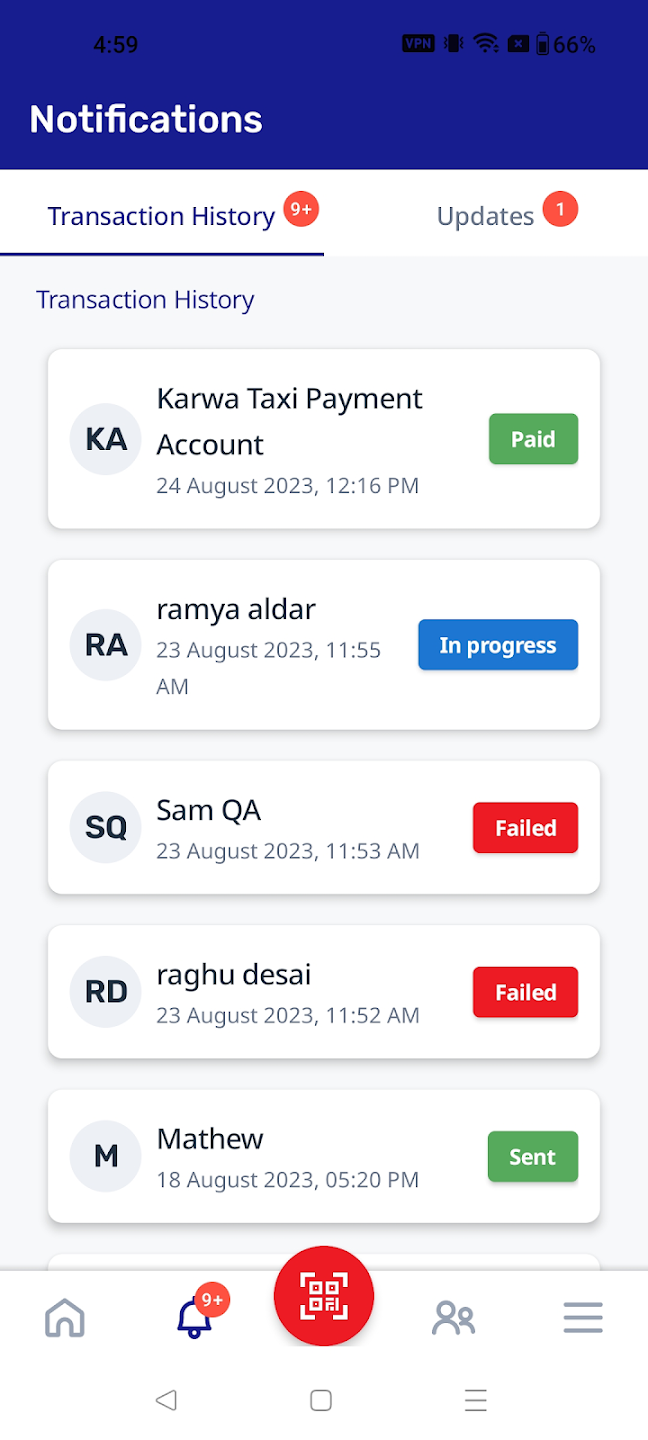
\includegraphics[width=\textwidth]{images/ooredoo_money_screenshot_3.png}
        \caption{Ooredoo Money Screenshot 3}
        \label{fig:ooredoo_3}
    \end{subfigure}
    \caption{Ooredoo Money Interface}
    \label{fig:ooredoo_interface}
\end{figure}

\textbf{Ooredoo Money:} Represented by the interface shown in Figure~\ref{fig:ooredoo_interface}, this Tunisian mobile payment solution offers digital wallet functionality with support for various retail transactions including bill payments, mobile top-ups, and merchant payments. It benefits from Ooredoo's extensive telecommunications infrastructure and has established partnerships with major Tunisian retailers across multiple categories. The platform provides basic QR code payment functionality and integration with some local banking systems.

However, Ooredoo Money faces significant limitations in comprehensive retail integration. It lacks sophisticated POS system compatibility, particularly with specialized retail management systems like ASM POS. The platform provides minimal corporate credit management features, making it unsuitable for employee benefit programs. Transaction processing can be slow during peak hours, and the vendor onboarding process is complex and time-consuming. Additionally, it offers limited real-time reporting capabilities for businesses and lacks advanced fraud detection mechanisms required for high-volume retail environments across diverse commercial sectors.

\clearpage

\subsubsection{International Solutions}

\begin{figure}[!htb]
    \centering
    \begin{subfigure}[b]{0.32\textwidth}
        \centering
        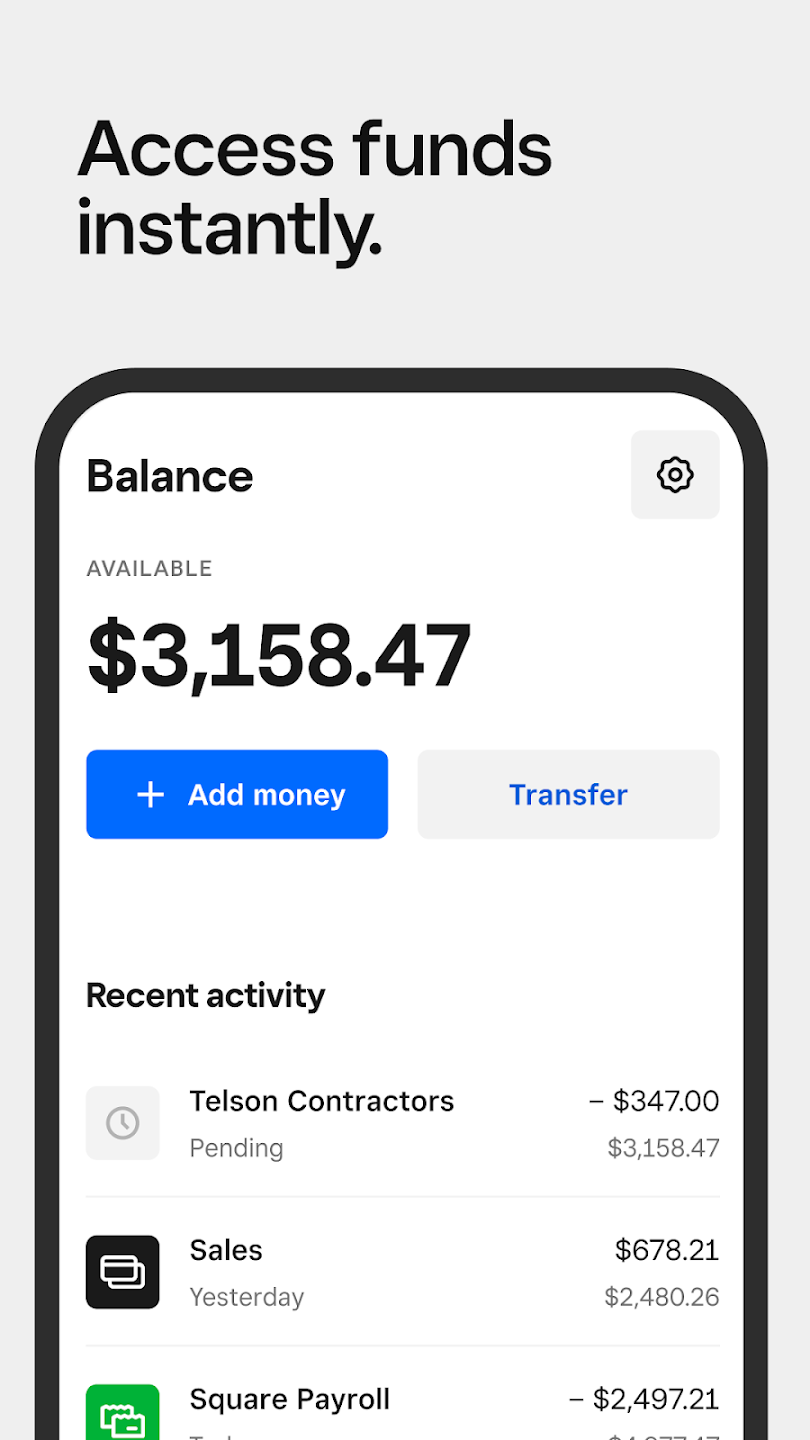
\includegraphics[width=\textwidth]{images/square_screenshot_1.png}
        \caption{Square Screenshot 1}
        \label{fig:square_1}
    \end{subfigure}
    \hfill
    \begin{subfigure}[b]{0.32\textwidth}
        \centering
        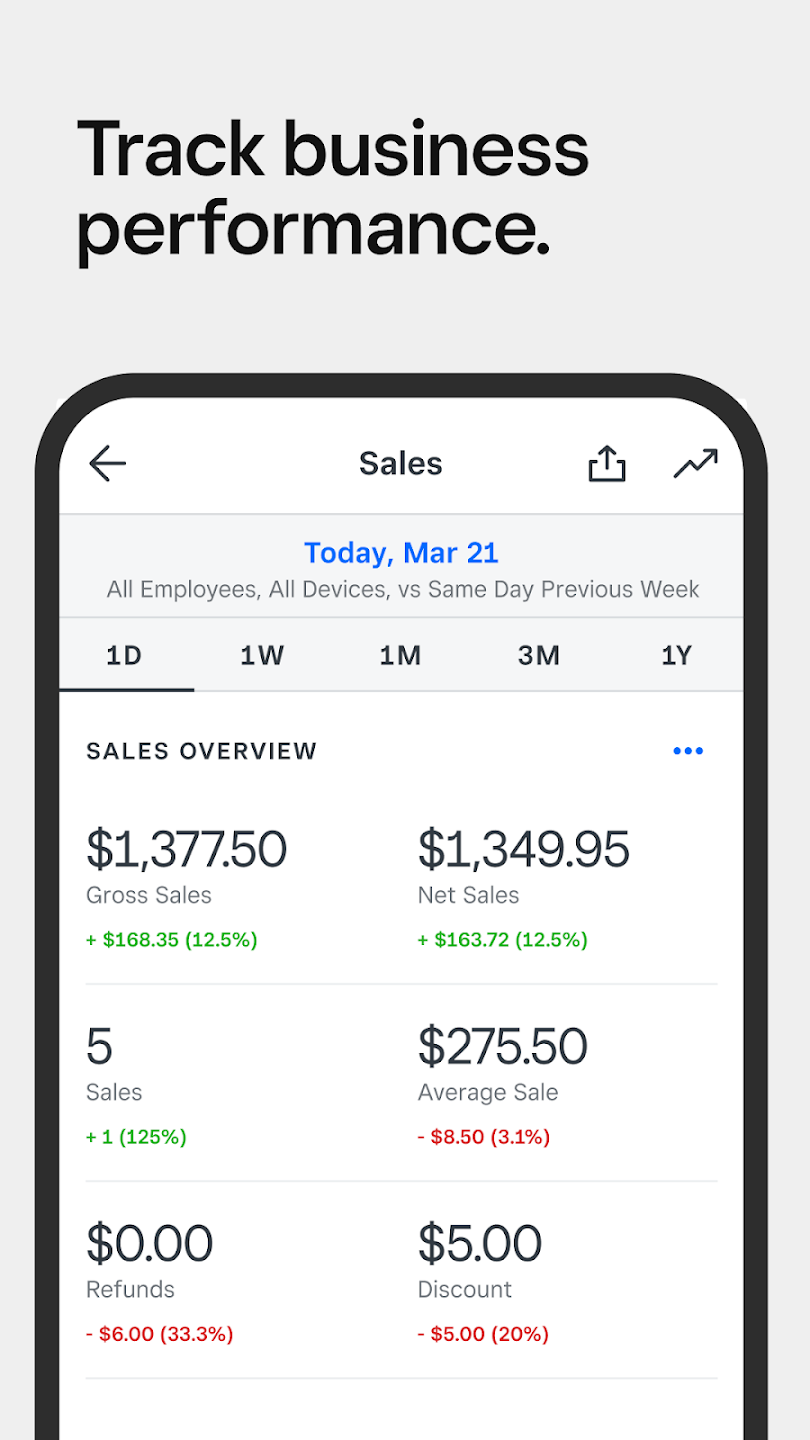
\includegraphics[width=\textwidth]{images/square_screenshot_2.png}
        \caption{Square Screenshot 2}
        \label{fig:square_2}
    \end{subfigure}
    \hfill
    \begin{subfigure}[b]{0.32\textwidth}
        \centering
        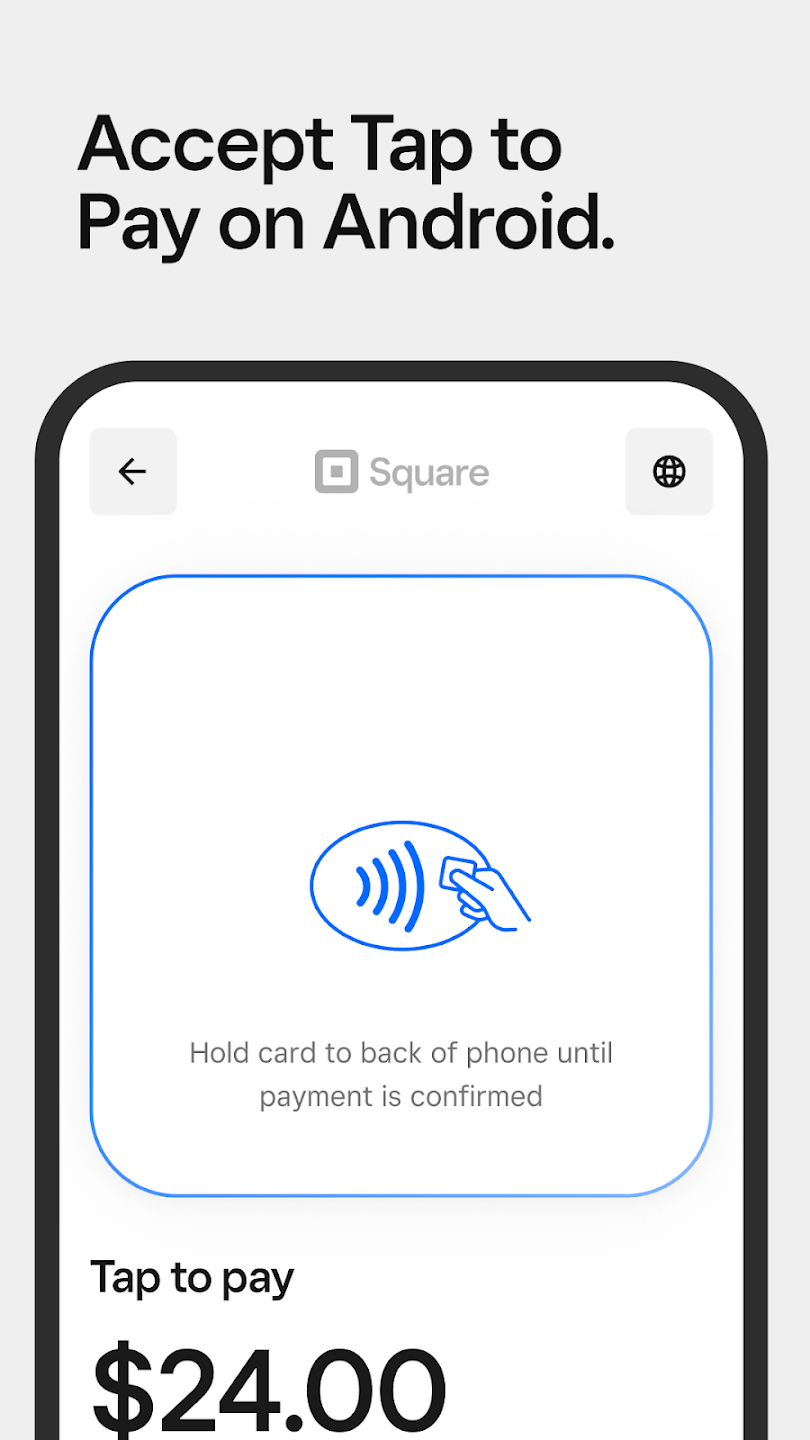
\includegraphics[width=\textwidth]{images/square_screenshot_3.png}
        \caption{Square Screenshot 3}
        \label{fig:square_3}
    \end{subfigure}
    \caption{Square POS Interface}
    \label{fig:square_interface}
\end{figure}

\textbf{Square:} Square (see Figure~\ref{fig:square_interface}) is a comprehensive international payment and POS solution serving millions of businesses worldwide across restaurants, retail stores, markets, boutiques, and service providers. The platform offers integrated hardware and software solutions with real-time payment processing, inventory management, and detailed analytics. It benefits from seamless integration across multiple retail categories, robust API ecosystem for third-party integrations, and comprehensive business management tools including payroll, invoicing, and customer relationship management.

However, Square's approach is primarily designed for direct merchant-customer transactions rather than corporate credit or employee benefit management. The platform lacks sophisticated corporate account management features, has no built-in employee spending controls or credit allocation systems, and provides minimal support for complex organizational hierarchies. Additionally, Square's pricing model can become expensive for high-volume transactions, and it has limited customization options for specific regional compliance requirements, particularly in emerging markets like Tunisia.

\clearpage

\begin{figure}[!htb]
    \centering
    \begin{subfigure}[b]{0.32\textwidth}
        \centering
        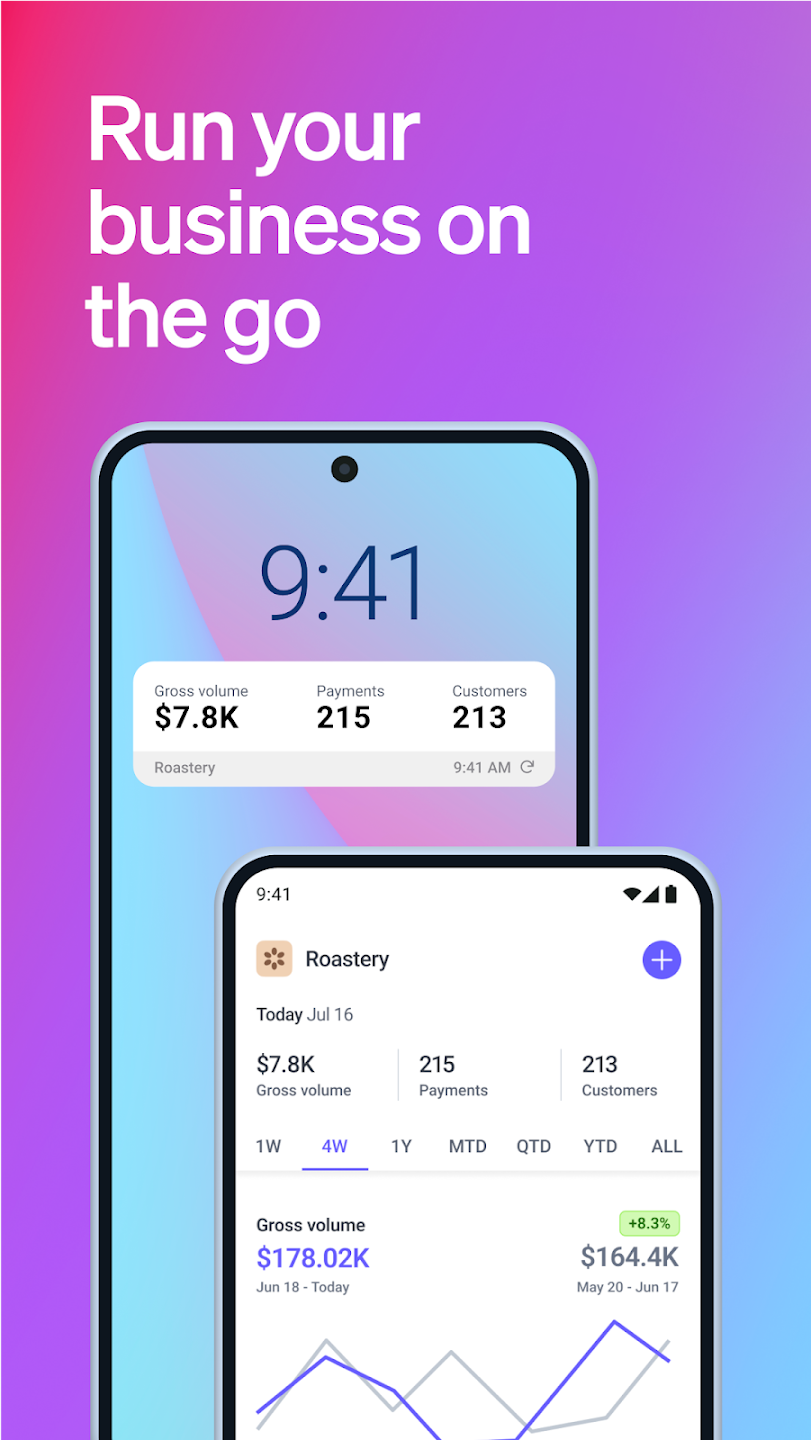
\includegraphics[width=\textwidth]{images/stripe_screenshot_1.png}
        \caption{Stripe Terminal Screenshot 1}
        \label{fig:stripe_1}
    \end{subfigure}
    \hfill
    \begin{subfigure}[b]{0.32\textwidth}
        \centering
        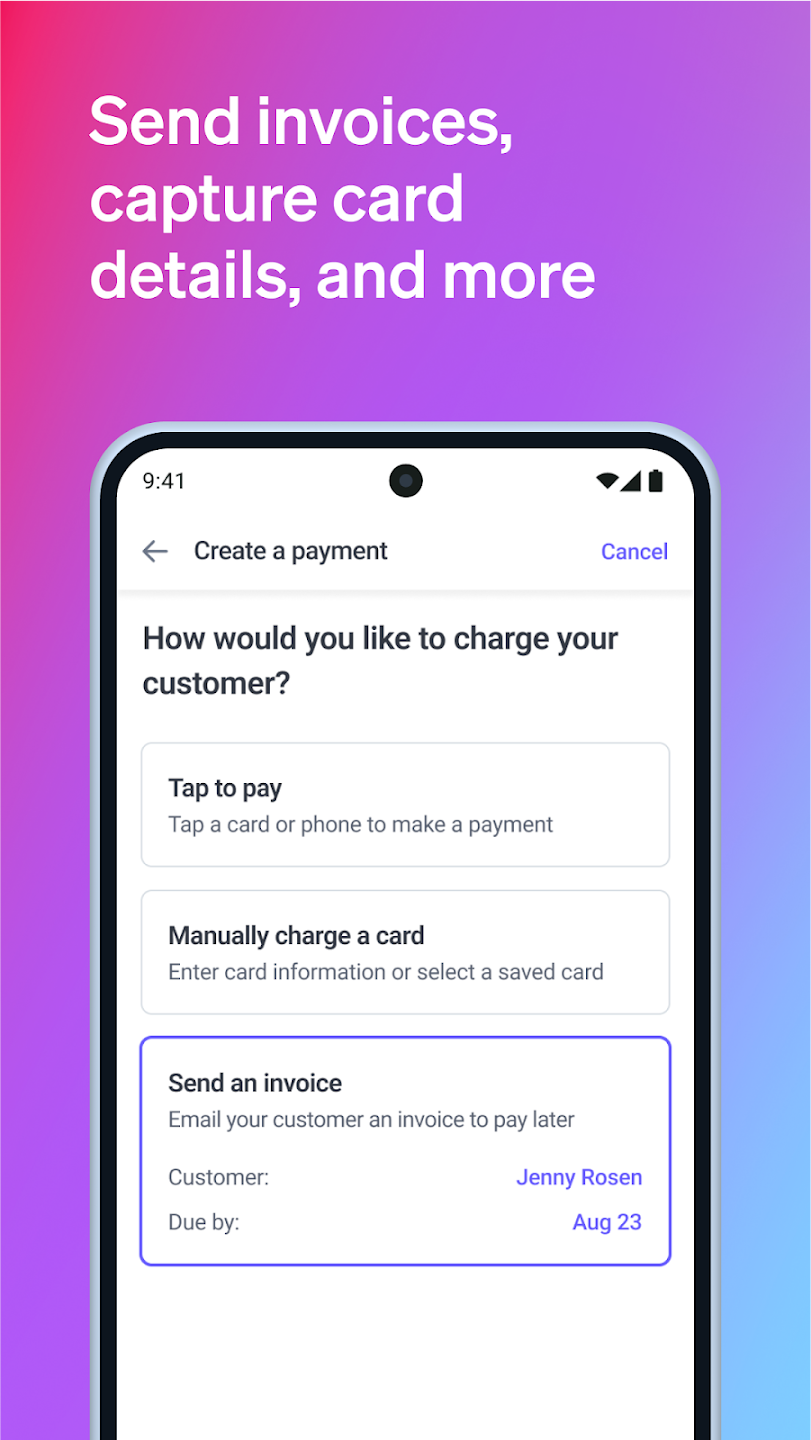
\includegraphics[width=\textwidth]{images/stripe_screenshot_2.png}
        \caption{Stripe Terminal Screenshot 2}
        \label{fig:stripe_2}
    \end{subfigure}
    \hfill
    \begin{subfigure}[b]{0.32\textwidth}
        \centering
        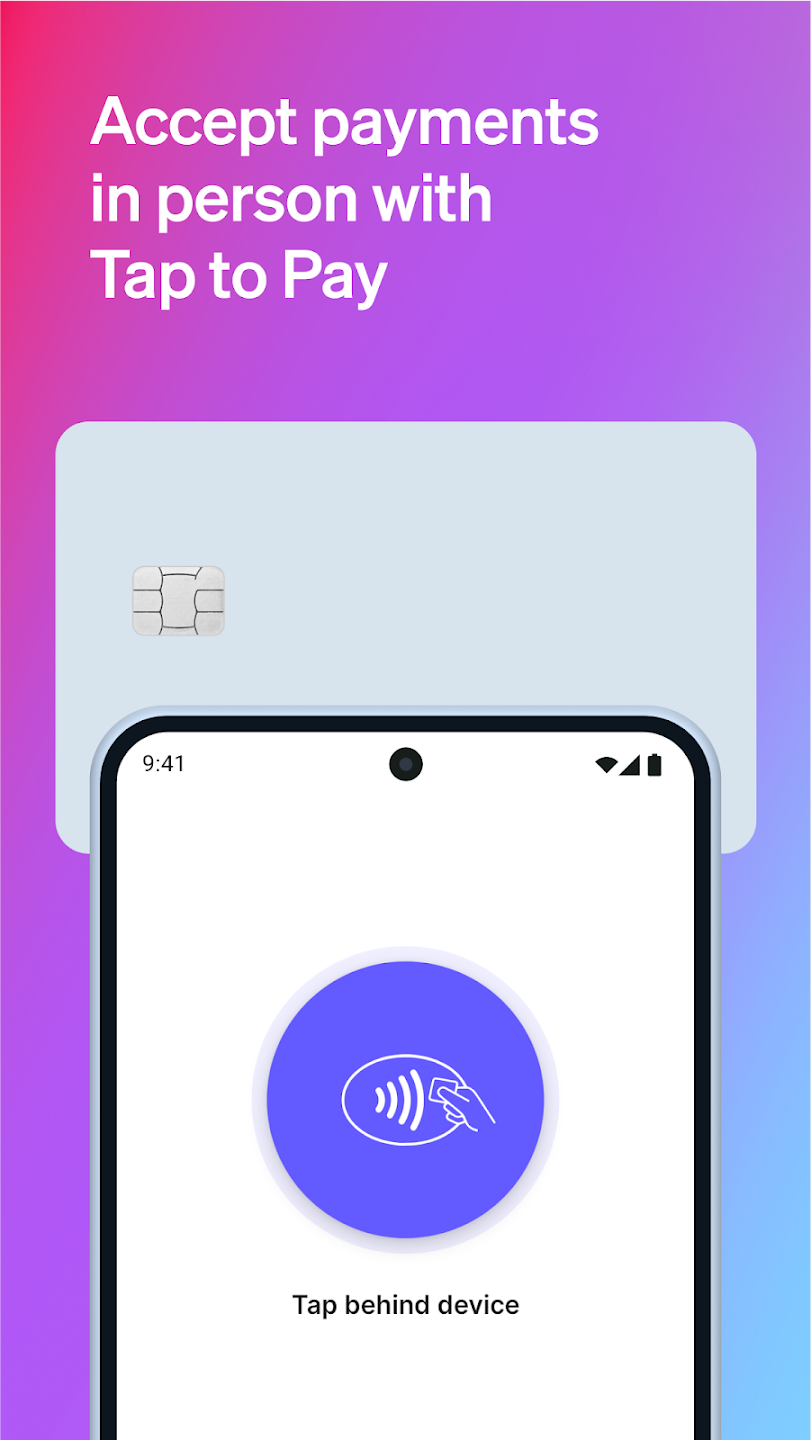
\includegraphics[width=\textwidth]{images/stripe_screenshot_3.png}
        \caption{Stripe Terminal Screenshot 3}
        \label{fig:stripe_3}
    \end{subfigure}
    \caption{Stripe Terminal Interface}
    \label{fig:stripe_interface}
\end{figure}

\textbf{Stripe Terminal:} Stripe Terminal (see Figure~\ref{fig:stripe_interface}) provides in-person payment capabilities as part of Stripe's comprehensive payment infrastructure, supporting businesses across retail, hospitality, healthcare, and professional services globally. The platform offers advanced payment processing with support for multiple payment methods, sophisticated fraud detection, and extensive API integration capabilities. It benefits from Stripe's robust global payment infrastructure, comprehensive developer tools, and seamless integration with e-commerce and in-store transactions.

Nevertheless, Stripe Terminal focuses primarily on payment processing rather than comprehensive retail management or corporate spending programs. The platform lacks built-in inventory management, employee benefit administration, and corporate credit allocation features. It requires significant technical expertise for implementation and customization, making it less accessible for smaller retailers. The system provides minimal out-of-the-box POS functionality and requires extensive third-party integrations for complete retail management. Furthermore, Stripe's services have limited availability in certain regions and may face regulatory constraints in emerging markets.

\subsubsection{General Critique}

This analysis has allowed us to identify the various approaches and functionalities offered by existing digital payment and retail transaction applications, both nationally and internationally. We have evaluated their strengths and limitations, with particular attention to multi-category retail support, POS system integration, corporate credit management, vendor onboarding processes, and cross-sector compatibility. Table~\ref{tab:summary_existing_study} below presents a synthesis of this comparison.

\begin{table}[!htbp]
    \caption{Summary of the Existing System Study}
    \centering
    \label{tab:summary_existing_study}
    \renewcommand{\arraystretch}{1.5}
    \begin{tabular}{|l|c|c|c|c|}
        \hline
        \textbf{Evaluation Criteria}
        & 
\includegraphics[width=2cm]{images/pluxee_logo.png}
        & 
\includegraphics[width=2cm]{images/ooredoo_money_logo.png}
        & 
\includegraphics[width=2cm]{images/square_logo.png}
        & 
\includegraphics[width=2cm]{images/stripe_logo.png} \\
        \hline
        Multi-Category Retail Support
        & \textcolor{red}{\ding{55}}
        & \textcolor{red}{\ding{55}}
        & \textcolor{green}{\ding{51}}
        & \textcolor{green}{\ding{51}} \\
        \hline
        Advanced POS Integration
        & \textcolor{red}{\ding{55}}
        & \textcolor{red}{\ding{55}}
        & \textcolor{green}{\ding{51}}
        & \textcolor{green}{\ding{51}} \\
        \hline
        Corporate Credit Management
        & \textcolor{red}{\ding{55}}
        & \textcolor{red}{\ding{55}}
        & \textcolor{red}{\ding{55}}
        & \textcolor{red}{\ding{55}} \\
        \hline
        User Experience / Interface Design
        & \textcolor{red}{\ding{55}}
        & \textcolor{red}{\ding{55}}
        & \textcolor{green}{\ding{51}}
        & \textcolor{green}{\ding{51}} \\
        \hline
        Real-time Transaction Processing
        & \textcolor{red}{\ding{55}}
        & \textcolor{red}{\ding{55}}
        & \textcolor{green}{\ding{51}}
        & \textcolor{green}{\ding{51}} \\
        \hline
        Vendor Onboarding Efficiency
        & \textcolor{red}{\ding{55}}
        & \textcolor{red}{\ding{55}}
        & \textcolor{green}{\ding{51}}
        & \textcolor{red}{\ding{55}} \\
        \hline
        Regional Compliance \& Availability
        & \textcolor{green}{\ding{51}}
        & \textcolor{green}{\ding{51}}
        & \textcolor{red}{\ding{55}}
        & \textcolor{red}{\ding{55}} \\
        \hline
    \end{tabular}
\end{table}

Based on these results, we can integrate best practices and address the identified shortcomings in the design of Credix, in order to precisely meet the expectations of diverse retail establishments, corporate clients, and end-users across multiple commercial sectors.